\chapter{基于细粒度变异的导向模糊测试技术研究}

模糊测试已被证明是一种非常强大的软件漏洞测试方法,是工业界和学术界研究的热点。
%在安全性重要性比较高的软件中,模糊测试发现了绝大多数远程程序执行漏洞和权限提升漏洞。
但是模糊测试一样有它的局限性,盲目的随机的变异测试用例很难到达测试程序的特定路径,导致一些漏洞很难被触发。
在源代码软件的漏洞挖掘中,一些可疑的漏洞触发点可以通过静态分析获取。所以,如何动态的产生测试用例到达可疑漏洞触发点是一项重要的研究内容。现有的主要的导向测试研究都是基于符号执行的\upcite{sparks_automated_2007, santelices_test-suite_2008, person_directed_2011, marinescu_katch:_2013, ma_directed_2011, haller_dowsing_2013, christakis_guiding_2016, bohme_regression_2013},又可称为导向白盒模糊测试。但是导向符号执行在程序分析和约束求解上耗费了大量的时间。在每一轮的测试中,为了到达目标区域,动态符号执行需要利用程序判断哪些分支需要反转,并沿着路径收集约束信息,最后调用约束求解器生成新的输入。而模糊测试不需要约束求解,仅仅通过变异生成测试输入。在相同的时间内,模糊测试产生的输入比动态符号执行高几个数量级。此外,符号执行还有其他的问题如环境交互问题和循环问题\upcite{baldoni_survey_2016}。Macel Bohme\upcite{bohme_directed_2017}提出了一种基于AFL(American fuzzy lop)\upcite{noauthor_american_nodate}的导向模糊测试工具AFL-go。此方法设计了一种用于衡量测试用例到目标区域的距离测度以及一种能量分配策略;随着测试时间的增加,AFL-go通过增加距离近的测试用例的变异次数,减少距离远的测试用例的变异次数,从而完成目标区域导向。但是AFL-go的变异还是具有盲目性,导向效率不高的缺点。
%不能规划测试用例的变异方向的缺点。
%从而导致导向效率不高。

本章提出了一种细粒度变异的导向模糊测试方法。该方法首先AFL-go收集测试用例;然后利用时间递归神经网络(Long Short-Term Memory,LSTM)训练出一个模型,用于判断哪些字段对靠近目标区域其关键作用,同时收集每个字段的权重;在动态运行测试用例之前,利用上述模型判断当前测试用例的关键字段并根据字段权重进行细粒度变异。本文方法能够更细粒度的变异指定字段,很大程度上消除AFL变异的盲目性,从而能够提高导向模糊测试的效率。


\section{反馈式模糊测试技术介绍}\label{模糊测试介绍}

模糊测试是现在最流行的软件测试技术,在很多复杂的程序中发现了很多安全漏洞。模糊测试的主要思想是不间断的产生新的畸形输入让程序执行,以期发现程序的未知行为、崩溃或者异常等行为。通常fuzzer(模糊测试工具)接受一组初始种子输入,通过随机变异或者其他的人为定义的变异策略产生大量的畸形输入反馈给程序执行,直到满足设定的停机条件。但是若遇到输入的格式特别复杂的情况,有时会需要产生数百万次的畸形输入的输入才能触发程序异常。

AFL(American fuzzy lop)\upcite{noauthor_american_nodate}是目前为止最先进的反馈式fuzzer,由Michał Zalewski于2015年开发完成并开源授予大众使用。相对于其他的fuzzer,AFL采用了多种数据变异策略和减少资源耗费的设置,并且不需要复杂的配置,能无缝的处理复杂真实软件,例如图像处理软件和文件压缩库软件。

AFL的优势主要在于其利用遗传算法对测试用例进行优化选择。
AFL维护一个种子测试用例队列,凡是能够提升代码覆盖率的测试用例都将作为种子测试用例,并且增加其新一轮的变异次数;反之,则丢弃。同时,该队列会通过一系列的筛选策略进行优化,以保证优先测试最优测试用例。AFL已经成功的在很多开源软件中发现了很多安全漏洞\upcite{baldoni_survey_2016},例如:Mozilla Firefox,ffmpeg,OpenSSL\upcite{noauthor_american_nodate}等。

AFL进行模糊测试测试的过程如算法\ref{AFL模糊测试}所示。算法输入为待测程序P、初始种子测试用例集以及每个样本的变异次数limit,第4到12行描述的是输入文件变异的详细过程,这里只描述了以字节为单位的变异。除了字节变异,AFL还包含如比特反转、随机替换/插入、已知字典、边界值等变异方式。另外,还采用了组合变异方法,将简单变异随机串联成为复杂变异,从而提高了变异样本覆盖新路径的能力。通过执行变异后的输入文件获取程序的结果result以及路径覆盖信息coverage(第13行);如果result是崩溃信息,则将其加入到MaliciousInputs中(第14-16行);如果路径覆盖coverage增加,则将对应输入input加入到种子序列中(第17-19行)。循环执行上述过程,直到时间耗尽(第21-23行)。

\begin{algorithm}
	\renewcommand{\algorithmicrequire}{\textbf{Input:}}
	\renewcommand{\algorithmicensure}{\textbf{Output:}}
	\caption{AFL模糊测试算法}
	\label{AFL模糊测试}
	\begin{algorithmic}[1]
		\REQUIRE seeds,待测程序 P,每个样本变异次数 limit
		\ENSURE 畸形测试用例 MaliciousInputs
		\STATE c1 = 0
		\FOR{seed in seeds}
			\WHILE{c1 < limit }
				\STATE input = seed
				\STATE length = len(seed)
				\STATE mutations = RandInt(length)
				\STATE mut = 0
				\WHILE{mut < mutations}
					\STATE byte = RandInt(length)
					\STATE mutate(input,byte)
					\STATE mut = mut+1
				\ENDWHILE
				\STATE result,coverage = execute(P,input)
				\IF{result is crash}
					\STATE MaliciousInputs.add(result)
				\ENDIF
				\IF{isIncreased(coverage)}
					\STATE seeds.add(input)
				\ENDIF
			\ENDWHILE
			\IF{timeout()}
				\STATE break
			\ENDIF
		\ENDFOR
	\end{algorithmic}
\end{algorithm}

AFL利用fork server机制增加执行效率。linux程序在执行到main函数之前会经过三个步骤:内核加载程序文件、调用libc\_start\_main以及初始化必要的数据结构和线程环境。一般的fuzzer在每次执行测试用例时都会完整的执行此三个步骤,造成模糊测试速度缓慢。而AFL在程序执行到main函数时,封存此时的状态,当程序再次执行测试用例时,利用linux的fork机制复制一个完全相同的进程,从而省略了上述的三个步骤。以执行binutils程序为例,AFL一秒钟能执行2000次个测试用例而一般的fuzzer只能执行不到100次。



\section{基本框架设计}

本文方法的目的是使用细粒度的变异方法尽快的生成能够到达目标区域的测试用例以挖掘漏洞或者验证程序的安全性。方法的前提条件有两个:(1)指定目标区域,在源代码中以危险操作语句的行数和文件名称表示(例如valid.c:6410);(2)LLVM bitcode插桩,用于编译时计算每个基本块到目标区域的距离,距离的定义见\ref{距离测度}节。

程序执行的路径由输入确定,所以若要控制程序执行到特定区域,相应的输入满足一定条件。图\ref{关键字段}是一个简单的示意图,右半部分是程序的执行路径,左半部分是程序的输入,若想要控制程序执行到关键区域$t$,则需要$x_1$和$x_3$满足一定条件;在本章方法中,$x_1$和$x_3$被称为关键字段。这里的字段是指测试用例中每个比特的位置。

\begin{figure}[htb]
\begin{center}
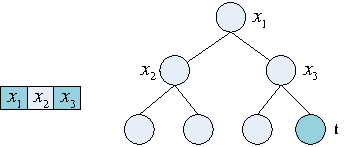
\includegraphics[scale=1.4]{关键字段}
\end{center}
\caption{关键字段解释}
\label{关键字段}
\end{figure}


细粒度导向模糊测试基本框架主要包括训练和测试两部分,如图\ref{细粒度导向fuzzing基本框架}所示。

训练的目的是产生一个模型;给定一个测试用例,此模型能够输出哪些关键字段能够使测试用例与目标区域的距离减小;同时训练计算每个关键字段的权重。初始测试用例经过变异生成新的不同的测试用例,此处变异为AFL的原始变异;测试用例通过执行引擎生成执行迹,计算每个执行迹到目标区域的距离,并与原始测试用例做比较;如果距离减小,则将测试用例改变的位置$x \oplus x^{'}$与相应的改变的距离输入到LSTM网络(Long Short Term)以训练模型;在利用LSTM网络训练的同时累积各个位置距离的变化值以计算权重。

测试的目的是利用训练的模型和字段权重引导模糊测试执行到目标区域。测试阶段的测试用例是训练阶段中与目标区域距离较小的一部分测试用例;利用基于字段权重的能量调度策略(\ref{基于字段权重的模糊测试能量调度策略}节)进行变异生成新的测试用例;经过执行引擎生成执行迹并测量距离,若距离减小则保留测试用例以待再次变异,反之丢弃,重复测试过程直到满足设定的停机条件。

\begin{figure}[htb]
\begin{center}
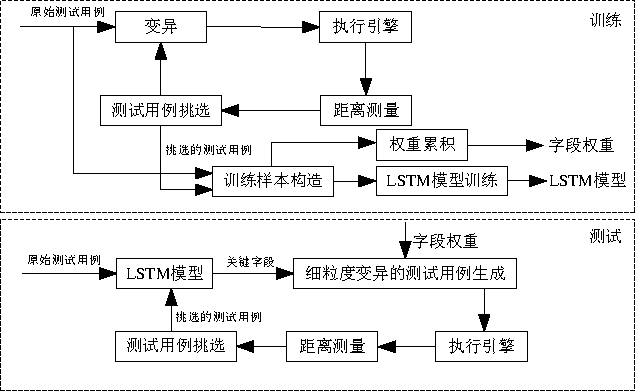
\includegraphics[scale=1.4]{细粒度导向fuzzing基本框架}
\end{center}
\caption{细粒度导向模糊测试基本框架}
\label{细粒度导向fuzzing基本框架}
\end{figure}

\section{基于LSTM的关键字段获取与权重计算}
\label{基于LSTM的关键字段获取}

本节对应图\ref{细粒度导向fuzzing基本框架}的训练部分,目的是获取对于距离减少起作用的关键字节区域,以及每个bit的权重,主要包括三个部分:衡量测试用例执行迹与目标区域距离的测度、基于LSTM的关键字段获取架构以及字段的权重计算。

\subsection{距离测度}
\label{距离测度}

本节采用AFL-go\upcite{bohme_directed_2017}的距离测度作为产生测试用例的工具。AFL-go是一个用于补丁测试和崩溃重现的工具,在静态分析的基础上能有效的调度AFL逼近目标区域,本章方法采用了其距离测度表示测试用例到目标区域的距离。其中,每一个目标区域在源代码中表示为一行代码,在软件的自动测试中,程序执行到某行代码和执行到对应的基本块意义相同,所以到某行代码的距离和到代码所在基本块的距离相同。

\subsubsection{函数距离}

函数距离指的是在函数调用图中两个函数的距离。函数$n$和$n^{'}$的距离记为$d_{f}(n,n^{'})$,表示在函数调用图中两函数之间边的数量。则函数$n$到目标函数集$T_f$之间的距离$d_f (n,T_f)$可以定义为$n$到$T_f$中所有函数距离的调和平均数,如式~(\ref{函数到目标函数集的距离})所示。

\begin{equation}\label{函数到目标函数集的距离}
s(X)=\left\{
\begin{aligned}
& undefined, & \text{如果} R(n, T_{f}) = \emptyset \\
& \lbrack \sum_{t_f \in R(n, T_{f})}d_{f}(n,t_{f})^{-1}\rbrack ^{-1} & \text{其他}
\end{aligned}
\right.
\end{equation} 

其中,$R(n,T_{f})$表示在$T_f$中和$n$具有可达关系的函数。调和平均数是总体各统计变量倒数的算术平均数的倒数。主要是用来解决在无法掌握总体单位数(频数)的情况下,只有每组的变量值和相应的标志总量,而需要求得平均数的情况下使用的一种数据方法。调和平均值的计算公式如式~(\ref{调和平均数})所示。相对于算术平均数,在多个目标情况下,调和平均能够区分距离一个目标较近离另外一个目标较远的点与多个目标中间点。如图\ref{调和平均数和算术平均值区别}所示,假设每个线段代表距离1,则中间三个点到$t_1$和$t_2$的算术平均值距离都是2;以调和平均数计算距离,如果一个点有一端比较靠近的某个目标,其距离比中间点的距离要小。本文方法的目标是要尽可能的到达目标区域,所以调和平均数较为合适。

\begin{equation}\label{调和平均数}
H_{n} = \frac{n}{\sum_{i=1}^{n}}
\end{equation}

\begin{figure}[htb]
\begin{center}
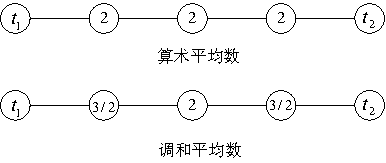
\includegraphics[width=10cm]{调和平均数和算术平均值区别}
\end{center}
\caption{调和平均数和算术平均值区别}
\label{调和平均数和算术平均值区别}
\end{figure}

\subsubsection{基本块距离}

虽然在程序的全局控制流图计算基本块的距离非常精确,但是全局的控制流图非常复杂,路径搜索和距离求解较为复杂,所以过程间、全局的基本块距离在这里使用过程内的基本块距离和函数距离去近似。如果函数距离越小,则函数之间的基本块的距离也越小。在一个函数$i$的控制流图$G_i$中,设定$d(m_1,m_2)$为$m_1$和$m_2$之间边的数量;$N(m)$为在基本块$m$中调用的函数中,与$T_f$函数具有可达关系的集合,即$N(m) = \{n | R(n, T_f) \neq \emptyset \}$;$T$表示在$G_i$中所有包含函数调用且此函数和$T_f$中函数具有可达关系,即$\forall m \in T.N(m) \neq \emptyset$。基于以上设定,每个基本块$m$与目标基本块集$T_b$的距离定义如式 ~(\ref{基本块到目标基本集的距离})所示。式中$c=10$是一个常量,用于放大函数之间的距离以近似基本块之间的距离,$d_{b}(m,Tb)$中的$m$表示所有的$G_i$中的任意的基本块,$G_i$函数调用图$CG$中任意函数的控制流图。

\begin{equation}\label{基本块到目标基本集的距离}
d_{b}(m,Tb)=\left\{
\begin{aligned}
& 0, & \text{如果} m \in T_{b} \\
& c \cdot \min\limits_{n \in N(m)}(d_{f}(n,T_{f})), & \text{如果} m \in T \\
& \lbrack \sum_{t \in T}(d_{b}(m,t) + d_{b}(t,T_{b}) ^{-1}\rbrack^{-1} & \text{其他}
\end{aligned}
\right.
\end{equation} 

\subsubsection{测试用例与目标区域之间的距离}

测试用例与目标区域之间的距离可以用程序执行测试用例产生的执行迹与目标基本块集的距离表示,距离越小越可能击中目标基本块。$\varphi(s)={b_1,b_2...b_n}$表示测试用例$s$的执行迹,$b_i$为程序执行的基本块。测试用例与目标区域之间的距离如式~(\ref{测试用例与目标区域之间的距离})所示。

\begin{equation}\label{测试用例与目标区域之间的距离}
d(s,T_b) = \frac{\sum_{m \in \varphi(s)} d_{b}(m,T_b) }{|\varphi(s)|}
\end{equation}

归一化后的测试用例与目标基本块集的距离如式~(\ref{归一化后的测试用例与目标区域之间的距离})所示。

\begin{equation}\label{归一化后的测试用例与目标区域之间的距离}
\hat{d}(s,T_b) = \frac{d_{b}(s,T_b)-minD }{maxD-minD}
\end{equation}
其中
\begin{equation}\label{minD和maxD的定义}
\begin{aligned}
& minD = \min\limits_{s_{i} \in S}\lbrack d(s_{i}, T_b) \rbrack \\
& maxD = \max\limits_{s_{i} \in S}\lbrack d(s_{i}, T_b) \rbrack
\end{aligned}
\end{equation}

归一化后,测试用例与目标区域之间的距离$\hat{d} \in [0,1]$。

\subsection{距离的获取方式}
AFL是运行非常快速的模糊测试器,如果在运行时动态测量测试用例到目标区域之间的距离会大大降低模糊测试的效率,所以本文采用在编译时将基本块之间的距离插桩到代码的方式来减少AFL动态运行负荷\upcite{bohme_directed_2017}。本文采用LLVM编译器对源码进行编译和插桩,用于距离测量的的静态插桩如图\ref{用于距离测量的的静态插桩}所示。

\begin{figure}[htb]
\begin{center}
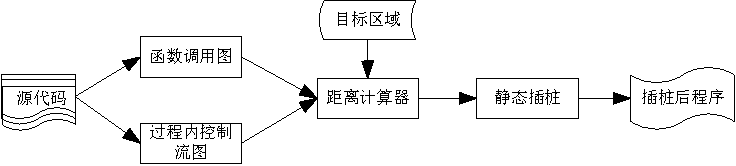
\includegraphics[scale=1.2]{用于距离测量的的静态插桩}
\end{center}
\caption{用于距离测量的的静态插桩}
\label{用于距离测量的的静态插桩}
\end{figure}

静态插桩的具体过程如下:

(1)产生程序的函数调用图和相应的过程内控制流图。函数调用图用函数声明表示;过程内控制流图用进入函数的第一个语句表示。二者通过编写相应的LLVM Pass生成。

(2)基本块之间的距离通过函数之间的距离以及过程内基本块的距离一起计算,详细的计算方式见\ref{距离测度}节。基本块之间距离的计算是通过调用Djikstra算法计算最短距离完成的。

(3)在每个基本块的跳转语句之后插入代码片段用于记录覆盖的控制流边。AFL使用64kb的共享内存存储边在执行过程中的遍历情况,每一条边对应一个字节。在64位的架构中,额外增加了另外16kb内存:8kb用于记录距离值另外8kb用于记录经过的基本块距离。静态插桩主要实现了两种功能:记录基本块到目标区域的距离以及将遍历的基本块记录到共享内存。

\subsection{训练过程}

\subsubsection{目标函数}

训练的目的是建立一个模型,给定一个测试用例,此模型能够输出一个位图用于表示哪些关键字段的改变能够使测试用例和目标区域的距离减少。因为测试用例是变长的,所以此模型可以被描述为一个函数簇,如式~(\ref{byte目标模型})所示。此函数簇的输入是任意数量的输入位置,输出的是各个位置的变异引起测试用例和目标区域距离减少的概率。

\begin{equation}\label{byte目标模型}
\{f_{k}: \{0x00, 0x01, ...,0xFF \}^{k} \rightarrow [0,1]^{k} | k \in N \}
\end{equation}

式~(\ref{bit目标模型})是以字节为单位判断是否有距离改变,但程序经常会用一个bit进行分支判断,所以本文进一步设定了bit级的目标函数,如式~(bit目标模型)所示。

\begin{equation}\label{bit目标模型}
\{f^{'}_{k}: \{0,1 \}^{8k} \rightarrow [0,1]^{8k} | k \in N \}
\end{equation}

在测试阶段,训练出的模型会首先根据当前测试用例相对于变异前的测试用例所改变的位置,去判断是否会引起距离的减少;若减少距离减少则执行此测试用例,反之丢弃,决策函数如式~(\ref{决策函数})所示。式中$x$表示测试用例,$x^{'}$表示变异后的测试用例,$\oplus$表示逐位异或运算,$(x \oplus x^{'})$表示测试用例变异的位置,$\alpha$是一个阈值,控制改变bit的最小数量。式~(\ref{决策函数})的主要思想是判断哪些关键bit上的改变才能够减小到目标区域的距离。

\begin{equation}\label{决策函数}
\sum_{k}(f^{'}(x \oplus x^{'})) > \alpha
\end{equation}

为了训练目标函数$f^{'}$,需要测试用例$x$,变异后的测试用例$x^{'}$,$x$到目标的距离$d(x)$以及$x^{'}$到目标之间的距离$d(x^{'})$;结合这四个参数可以设定一个生成一个有监督的数据集,如式~(\ref{训练集})所示。

\begin{equation}\label{训练集}
xy = \{(x, x \oplus x^{'}) | \bigtriangleup (d(x),d(x^{'})) > 0 \}
\end{equation}

\subsubsection{训练模型选择}

因为测试用例的长度是可变的,且bit之间存在关联,本文使用循环神经网络(Recurrent Neural Network,RNN)训练决策函数。RNN非常适用于处理像程序测试用例这样的序列数据\upcite{rodriguez_recurrent_1999}。因为RNN的记忆功能,所以RNN在处理有格式的文件输入时非常有用。RNN已经成功的应用于统计机器翻译当中\upcite{cho_learning_2014,bahdanau_neural_2014},本章要处理的问题和此相似,因为测试用例也可以当做是一种语言。

但是RNN很难处理较长的序列,所以本文采用时间递归神经网络(Long Short-Term Memory,LSTM)。相对于RNN,LSTM在最顶层增加了一条名为”cell state“的信息传送带同时,所以能够处理更长的序列。同时,LSTM丢弃超过生命周期的序列记忆,以增加处理更长序列的能力。LSTM的一个循环单元(recurrent unit)的状态更新和输出如式~(\ref{循环单元})所示。

\begin{equation}\label{循环单元}
h_{t}, o_{t} = f(x_{t},h_{t-1})
\end{equation}

将式~(\ref{循环单元})分解,如下式~(\ref{LSTM分解})所示。其中,$\sigma$是Sigmoid函数,$W_{*}$为学习的权重向量,$b_{*}$是学习的误差向量。$f_t$是忘记门层,$i_t$是输入门层二者决定是否保留或者丢弃当前输入。通过三种门交织处理使得LSTM能够处理更长的序列。

\begin{equation}\label{LSTM分解}
\begin{aligned}
& f_{t} = \sigma(W_{f} \centerdot [x_{t}, h_{t-1}] + b_f) \\
& i_t = \sigma (W_{i} \centerdot [x_{t}, h_{t-1}] + b_{i}) \\
& C_{t} = f_{t} \times C_{t-1} + i_{t} \times tanh(W_C \centerdot [x_{t}, h_{t-1}] + b_{C}) \\
& o_t = \sigma(W_{o} \centerdot [x_{t}, h_{t-1}] + b_{o}) \\
& h_{t} = o_{t} \times tanh(C_{t})
\end{aligned}
\end{equation}

\subsubsection{关键字段权重计算}
\label{关键字段权重计算}

本文用一个哈希表存储所有bit改变引起的距离的改变,每个bit的权重计算如~(\ref{bit权重计算})所示。其中,$x$和$x^{'}$表示变异前测试用例和变异后的测试用例,$sum(x \oplus x^{'})$表示$x^{'}$相对于$x$变化的字节数量,$\bigtriangleup (d(x),d(x^{'})$表示$x^{'}$相对于$x$减少的距离。式~(\ref{bit权重计算})表示将$\bigtriangleup (d(x),d(x^{'})$平均的分配在改变的每个bit上。训练结束后将权重累积到所有bit位置上,对权重进行归一化,得到bit权重的最终结果。

\begin{equation}\label{bit权重计算}
\omega^{k}_{i}=\left\{
\begin{aligned}
& \omega_{i} = \bigtriangleup (d(x),d(x^{'}))/sum(x \oplus x^{'}), & \text{如果 } i \in \{ x \oplus x^{'} \}\\
& 0 & \text{其他}
\end{aligned}
\right.
\end{equation} 

\begin{equation}\label{bit权重累积}
\omega_{i} = \sum_{k=1} \omega^{k}_{i}
\end{equation}

在实际训练的过程中,并不是所有的bit的权重都不相同,本文将具有相同bit权重的bit集合称之为bit集。

\subsubsection{关键字段权重与程序执行路径的关系}

本节利用程序Listing \ref{权重与程序执行路径的关系实例程序}论述关键字段权重与程序执行路径之间的关系。图\ref{字段权重和程序执行路径的关系}是Listing \ref{权重与程序执行路径的关系实例程序}的执行树,每个节点代表一个基本块,第6行的代码和图中红色节点相对应,这里将此基本块表示为$t$;叶子节点下面的字符($a,b,c,d,e,f,g,h$)代表的是执行到相应节点的路径。若要执行$h$,需要的条件是$x1>0 \wedge x3>100 \wedge x7>100$。

假设当前的测试用例$s=(-1,-2,1,-200,1,1,1)$,执行的路径是$a$,按照\ref{距离测度}节的距离计算方式,$d(s,a) = 3$。任意修改$x2,x4,x5$所生成新测试用例$s^{'}$,其与h的距离$d(s,s^{'})$都不会减少。若要减少到h的距离,$x1$必须要大于0,如此$x1$的权重则会增加,$x1$的权重一定大于$x2,x4,x5$。$s$经过变异后生成$s^{'}=(1,-2,1,-200,1,1,1)$,执行的路径是e。对于$s^{'}$,若要减少到h的距离就必须要变异$x3$,从而导致$x3$的权重增加。

在对大量样本进行训练的情况下,关键字段权重能够反应测试用例和输入的关系,即权重大的字段能够控制执行树的节点。对于每一个测试用例,根据其关键字段的权重能够更容易的到达目标区域。

\begin{lstlisting}[language=C,caption=权重与程序执行路径的关系实例程序,label=权重与程序执行路径的关系实例程序]
void f(int x1, int x2, int x3, int x4, int x5, int x6, int x7)
{
	if(x1 > 0){
		if(x3 > 10){
			if(x7 > 100)
				target();
		}else{
			if(x6 > 15){
				normal();
			}else
				normal();
		}
			
	}else{
		if(x2 < -1){
			if(x4 < -125){
				normal();
			}else
				normal();
		}else{
			if(x5 < -256){
				normal();
			}else
				normal();
		}
	}
}
\end{lstlisting}

\begin{figure}[htb]
\begin{center}
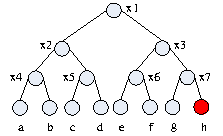
\includegraphics[scale=3]{字段权重和程序执行路径的关系}
\end{center}
\caption{Listing \ref{权重与程序执行路径的关系实例程序}的执行树}
\label{字段权重和程序执行路径的关系}
\end{figure}


\section{动态测试}
\label{基于字段权重的模糊测试能量调度策略}

本节重点论述在AFL的原有能量调度基础上,基于关键字段和模拟退化算法设计能量调度策略。本章使用的能量的含义是指模糊测试中对一个测试用例的变异次数。

\subsection{细粒度变异的测试用例生成过程}

图\ref{细粒度变异的测试用例生成过程}是本文采用的通过细粒度变异生成测试用例的过程。对于测试用例$s$,LSTM模型输出使距离减少的bit集,对照全局权重表形成归一化后的bit集,每个bit集的权重用$\omega^{'}_{i}$表示。对于每一个测试用例基于模拟退火框架生成一个能量$p$,按照bit集的权重重新计算每个bit集的权重$p_i$,能量越大表明该bit集变异的次数越多。通过对靠近目标区域的测试用例分配更多的能量,以及对每个bit集根据权值进行细粒度变异能够使测试用例以更大的可能性更快的到距离更近的测试用例,以此增加导向性模糊测试的效率。

\begin{figure}[htb]
\begin{center}
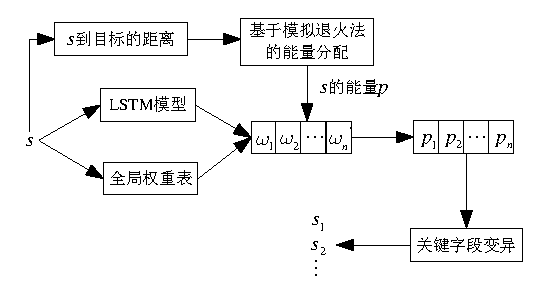
\includegraphics[scale=1.4]{细粒度变异的测试用例生成过程}
\end{center}
\caption{细粒度变异的测试用例生成过程}
\label{细粒度变异的测试用例生成过程}
\end{figure}


\subsection{细粒度变异能量分配策略}

AFL通过测试用例的执行时间、覆盖的基本块数量以及测试用例的深度(测试用例相对与初始测试用例变异的次数)来决定当前测试用例的能量。AFL初始的能量分配策略是以代码覆盖率为导向的,并不适合特定目标导向。本节基于字段权重,介绍一种模拟退火框架的能量分配策略。此策略的主要思想是对距离目标区域较近的测试用例变异能更容易击中目标区域。具体实施时,为距离目标区域较近的测试用例分配更高的能量,从而能以更高的可能性生成到达目标区域的测试用例。

模拟退火法\upcite{kirkpatrick_optimization_1983}的出发点是基于物理中固体物质的退火过程与一般组合优化问题之间的相似性。模拟退火算法从某一较高初温出发,伴随温度参数的不断下降,结合概率突跳特性在解空间中随机寻找目标函数的全局最优解,即在局部最优解能概率性地跳出并最终趋于全局最优。模拟退火算法是一种通用的优化算法,理论上算法具有概率的全局优化性能。温度是模拟退火的一个重要参数,随着温度的降低,较差解决方案的接受率也降低。在算法开始运行时,初始温度$T=T_0=1$,此时算法接受较差解决方案的概率较高,当$T$接近于0时,算法退化为经典的梯度下降算法。

将模拟退火算法的框架应用到导向模糊测试中想要达到的效果是:测试开始时即温度较高时,允许以较高的概率变异那些距离目标区域较远测试用例,随着时间的推移这种概率越来越低,到时间趋于无穷时只变异距离目标区域最近的测试用例。现在最流行的冷却方案是指数冷却方案\upcite{kirkpatrick_optimization_1983},如式~(\ref{模拟退火算法})所示。其中,$\alpha<1$是个常量,$\alpha$的区间为$[0.8,0.99]$。

\begin{equation}\label{模拟退火算法}
T_{exp} = T_0 \centerdot \alpha^{k}
\end{equation}

在用模糊测试方法挖掘漏洞时,一定会设定一个时间限制$t_x$。在使用模拟退火框架设计能量分配策略时,也需要设定一个$t_x$。在$t_x$之前是导向模糊测试的搜索路径阶段,在此阶段分配给距离较远的测试用例较大的能量,以搜索更多的路径。在$t_x$之后导向模糊测试进入收敛阶段,在此阶段分配给距离最近的测试用例的能量几乎达到最大,使产生的测使用例更好的逼近目标区域。在到达$t_x$时,模拟退火算法等价于梯度下降算法,距离目标区域最近的测试用例分配的最高的能量,让AFL着重变异和测试最有希望击中目标区域的测试用例。假设设置经过$k$轮的迭代之后$T_{exp}=0.1$,则在时间$t$的温度$T_exp$可以通过式~(\ref{t时间温度的计算})的推导获得。同样,可以将$T_{exp}$设置为其他的值,$T_{exp}$越小温度降低的越快。

\begin{equation}\label{t时间温度的计算}
\begin{aligned}
& \alpha^{k_{l}} = 0.1 & \text{当经过}k_{l}\text{轮迭代之后}\\
& k_{l} = log(0.1)/log(a) &\text{求解}k_{l}\\
& T_{exp} = \alpha^{t/t_{x} \centerdot (log(0.1)/log(a))} & \text{将}k_{l}\text{代入}\\
& T_{exp} = 10^{-t/t_{x}} &\text{化简}
\end{aligned}
\end{equation}

模拟退火的温度参数随着时间的增加而减少的,而基于模拟退火框架的能量分配的目的是距离近的测试用例的能量随着时间的增加越来越高,距离大的测试用例的能量随时间的增加越来越低。所以在式~(\ref{t时间温度的计算})的基础上可定义模拟退火的能量分配如式~(\ref{基于模拟退火的能量分配})所示。其中$c_{1}$是一个可调节的常量,控制着搜索阶段距离大的测试用例所分配的能量,$c_{1}$越大距离大的测试用例能量越大。典型的,可以设置$c_{1} = 0.5$;在开始测试时测试距离为1的测试用例的能量为0.5。

\begin{equation}\label{基于模拟退火的能量分配}
\begin{aligned}
& p(m,T_{b}) = (1- \hat{d}(s,T_{b})) \centerdot (1-T_{exp}) + c_{1}T_{exp}
\end{aligned}
\end{equation}

在式~(\ref{基于模拟退火的能量分配})的基础上,可定义每个bit集的变异能量如式~(\ref{关键字段能量})所示,其中,$\omega^{'}_{i}$测试用例关键字段中每个bit的权重。

\begin{equation}\label{关键字段能量}
p_{i} = \frac{\omega^{'}}{\sum_{i} \omega^{'}} \centerdot p(m,T_{b})
\end{equation}

将式~(\ref{关键字段能量})应用到AFL原有的能量策略上,最终的能量分配如式~(\ref{最终能量分配})所示。其中,$c_{2}$是一个常量,用于控制不同距离的能量分配,$c_{2}$越大,距离大的测试用例分配的能量越小,此数值可以在测试时根据不同的目的具体调整。

\begin{equation}\label{最终能量分配}
\hat{p}_{i} = p_{afl}(s) \centerdot 2^{10(p_{i}-c_{2})}
\end{equation}

\section{实验结果与分析}

\subsection{实验设计}

(1)实验目的

为了测试基于细粒度变异的导向模糊测试方法的有效性,本节在测试效率以及已知漏洞的挖掘数量两个方面上进行了实验。

(2)实验环境

%本节主要针对两个目标程序进行实验:readelf\upcite{noauthor_gnu.org_nodate}和libxml2\upcite{noauthor_xml_nodate}。readelf是Linux下binutils中用于分析ELF文件的命令,libxml2是一个XML的C语言解析器和工具库。本实验测试的readelf对应的binutils版本是2.28,libxml2版本是2.9.4,测试软件的基本情况如表\ref{测试软件基本信息}所示。根据CVE数据库的记录libxml2.9.4包含6个漏洞,readelf包含14个漏洞。除了将这些漏洞发生的代码行作为导向的目标区域,还在libxml2的代码中随机标记了42行代码,在readelf代码中随机标记了36行代码作为目标区域。本实验将就目标区域的覆盖数量、目标区域的击中次数以及漏洞的发现数量作为标准衡量本文方法的有效性。

本节主要针对readelf\upcite{noauthor_gnu.org_nodate}进行实验。readelf是Linux下binutils中用于分析ELF文件的命令,本实验测试的readelf对应的binutils版本是2.28,测试软件的基本情况如表\ref{测试软件基本信息}所示。根据CVE数据库的记录readelf包含14个漏洞。除了将这些漏洞发生的代码行作为导向的目标区域,还在readelf代码中随机标记了36行代码作为目标区域。本实验将就目标区域的覆盖数量、目标区域的击中次数以及漏洞的发现数量作为标准衡量本文方法的可行性和有效性。

\begin{table}[ht]
\begin{center}
\caption{测试软件基本信息}
\label{测试软件基本信息}
\begin{small}
\begin{tabular}{|l|l|l|l|}
\hline
{\bf 软件版本} & {\bf CVE-ID} & {\bf CVE数量} & {\bf 总标记数量} \\
\hline
readelf2.28 & CVE-2017-14333,CVE-2017-15996,CVE-2017-16830 & &\\
& CVE-2017-6965,CVE-2017-6966,CVE-2017-6969 & & \\
& CVE-2017-7209,CVE-2017-8398,CVE-2017-9038 & & \\
& CVE-2017-9039,CVE-2017-9041,CVE-2017-9042 & & \\
& CVE-2017-9043 CVE-2017-9044 & 14 & 50\\
\hline
\end{tabular}
\end{small}
\end{center}
\end{table}

本实验使用Keras\upcite{chollet_keras:_2017}作为前端训练预测模型,选择Tensorflow\upcite{abadi_tensorflow:_2016}作为Keras的底层后端。因为训练测试用例的长度是不同的,而且存在非常大的测试用例一个输入文件可能达到200KB,所以本实验将大于10KB的文件以10KB为单位进行分段。本试验采用Nvidia GTX970 GPUs训练12小时,使用绝对平均误差(Mean Absolute Error,MAE)作为损失函数,使用Adam优化器\upcite{kingma_adam:_2014}以$5 \times 10^{-5}$的学习率训练模型。训练模时可以设定不同的输入输出文件大小,本实验采用的是64bit。

动态导向模糊测试使用的是Inter Xeon CPU E3-1231 v3 @ 3.40GHz,16G RAM,实验设定的搜索路径时间为8小时,8小时后的时间为目标区域导向时间。

(3)实验过程

本实验的实验过程如图\ref{细粒度导向fuzzing基本框架}所示,首先训练与距离相关的关键字段以及关键字段的权重,然后进行动态模糊测试。
本实验的训练所使用的测试用例是由AFL-go产生。刚开始测试时需要搜索更多的路径,所以在运行AFL-go时将式~(\ref{基于模拟退火的能量分配})中的$c_1$设为0.6,给予距离大的测试用例更大的能量,式~(\ref{最终能量分配})中的$c_2$参数设为0.5。本实验运行了AFL-go 6个小时来收集用于训练的样本。将收集的样本按照距离的大小排序,将距离等距的划分为10个区间,即$[0,0.1),[0.1,0.2)...[0.9,1]$。对落入每个区间的测试用例随机的抽取20\%。训练时,每次不放回式抽取两个测试用例,提取每个测试用例与目标区域的距离,按照式~(\ref{构造训练集})构造样本$xy$。

\begin{equation}\label{构造训练集}
xy = \{(x,x \oplus x^{'}) | |d(x,x^{'})| > 0\}
\end{equation}

在动态模糊测试阶段,针对每个测试用例,LSTM模型会输出需要变异的关键字段。关键字段结合全局字段权重表,用于指导字段变异和能量调度,从而近一步指导动态模糊测试的导向性。

\subsection{结果分析}

AFL在判断测试用例是否重复时使用两个标准:(1)程序在执行不同测试用例经过的基本块不相同;(2)经过的基本块相同,但遍历基本块的次数不相同。对于一些有漏洞的危险区域,即使程序执行到目的基本块也不能保证能触发漏洞,例如由循环写造成的缓冲区溢出漏洞,触发此类型的漏洞就需要多次遍历循环内部的基本块。所以可以认为,在测试用例经过的基本块不变的情况下,若能够增加目的区域的遍历次数就更可能触发漏洞。本节将这种能够到达目标区域,经过的基本块相同,但是执行的次数不同的测试用例称为非重复击中目标区域测使用用例。图\ref{非重复击中目标区域测试用例数量对比}是本章方法、AFL-go以及AFL的非重复击中目标区域测使用用例数量的对比。

从图\ref{非重复击中目标区域测试用例数量对比}上可以看出,在8小时之后本章方法和AFL-go非重复击中目标区域测试用例数量增加的速率明显增加,而原始的AFL则没有显著提高。经过24小时本章方法的非重复击中目标区域测试用例数量达到了213个,而AFL-go只达到了127个,AFL只有28个。从非重复击中目标区域测试用例的增加速率以及总数量来看,本章方法要优于AFL-go和AFL。

\begin{figure}[htb]
\begin{center}
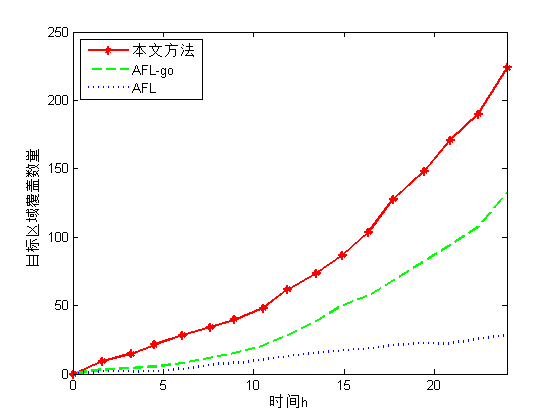
\includegraphics[scale=0.9]{非重复击中目标区域测试用例数量对比}
\end{center}
\caption{非重复击中目标区域测试用例数量对比}
\label{非重复击中目标区域测试用例数量对比}
\end{figure}

图\ref{目标区域覆盖数量对比}是本章方法、AFL-go以及AFL工具在测试readelf时,对标记的50个区域的覆盖情况。从图\ref{目标区域覆盖数量对比}可以看出本章方法和AFL-go在引导模糊测试到达目标区域时具有显著的优势。在8个小时之后,导向目标区域的速率明显增加。本章方法在运行了17小时36分钟之后能够覆盖35个目标区域,AFL-go在执行了22小时21分钟之后覆盖了24个目标区域,而原始的AFL在24个小时之后只能覆盖4个目标区域。实验表明,本章方法在导向目标区域的速率以及覆盖目标区域的数量比AFL-go有明显的提高。

\begin{figure}[htb]
\begin{center}
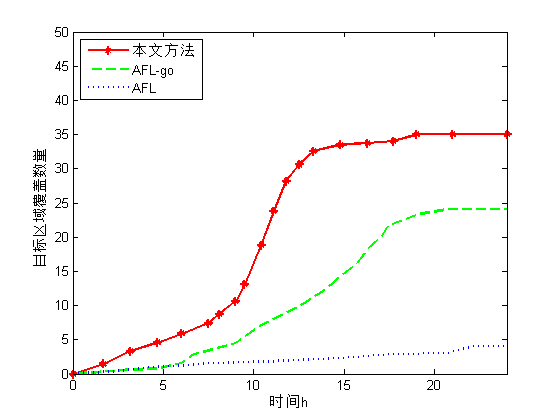
\includegraphics[scale=0.9]{目标区域覆盖数量对比}
\end{center}
\caption{目标区域覆盖数量对比}
\label{目标区域覆盖数量对比}
\end{figure}

图\ref{发现漏洞数量对比}是本章方法、AFL-go以及AFL工具在测试readelf测试漏洞数量的对比情况。从图\ref{发现漏洞数量对比}可以看出,AFL在24个小时之内没有发现任何漏洞,而在指定目标区域后,本章方法和AFL-go发现的漏洞数量显著增加。本章方法在运行16小时38分钟后发现了11个漏洞,AFL-go在运行了19个小时25分钟后发现了6个漏洞;本章方法在5小时31分钟时发现了第一个漏洞,而AFL-go在8小时13分钟发现了第一个漏洞;说明经过一段时间的路径探索之后本章方法能更早更快的发现漏洞,且最终发现的漏洞比AFL-go多出3个。
\begin{figure}[htb]
\begin{center}
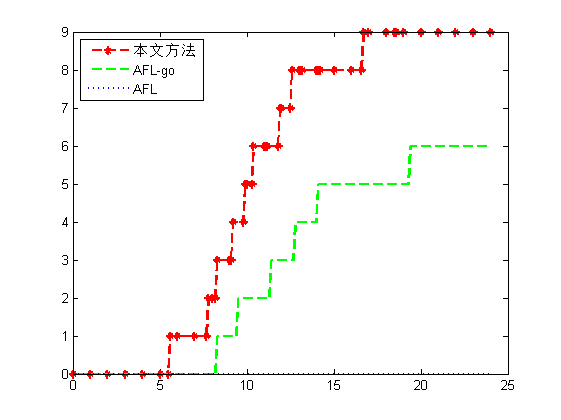
\includegraphics[scale=0.9]{发现漏洞数量对比}
\end{center}
\caption{发现漏洞数量对比}
\label{发现漏洞数量对比}
\end{figure}

\section{本章小节}

本节提出了一种基于细粒度变异的导向模糊测试方法。该方法首先AFL-go收集测试用例;然后利用时间递归神经网络(Long Short-Term Memory,LSTM)训练出一个模型,用于判断哪些字段对靠近目标区域其关键作用,同时收集每个字段的权重;在动态测试测试用例之前,利用上述模型判断对于当前测试用例哪些是关键字段并根据字段权重定向的变异。本章方法能够更细粒度的变异制定的字段,很大程度上消除AFL变异的盲目性,从而能够提高导向模糊测试的效率。